\section{Operation}

\begin{figure}[H]
  \centering
  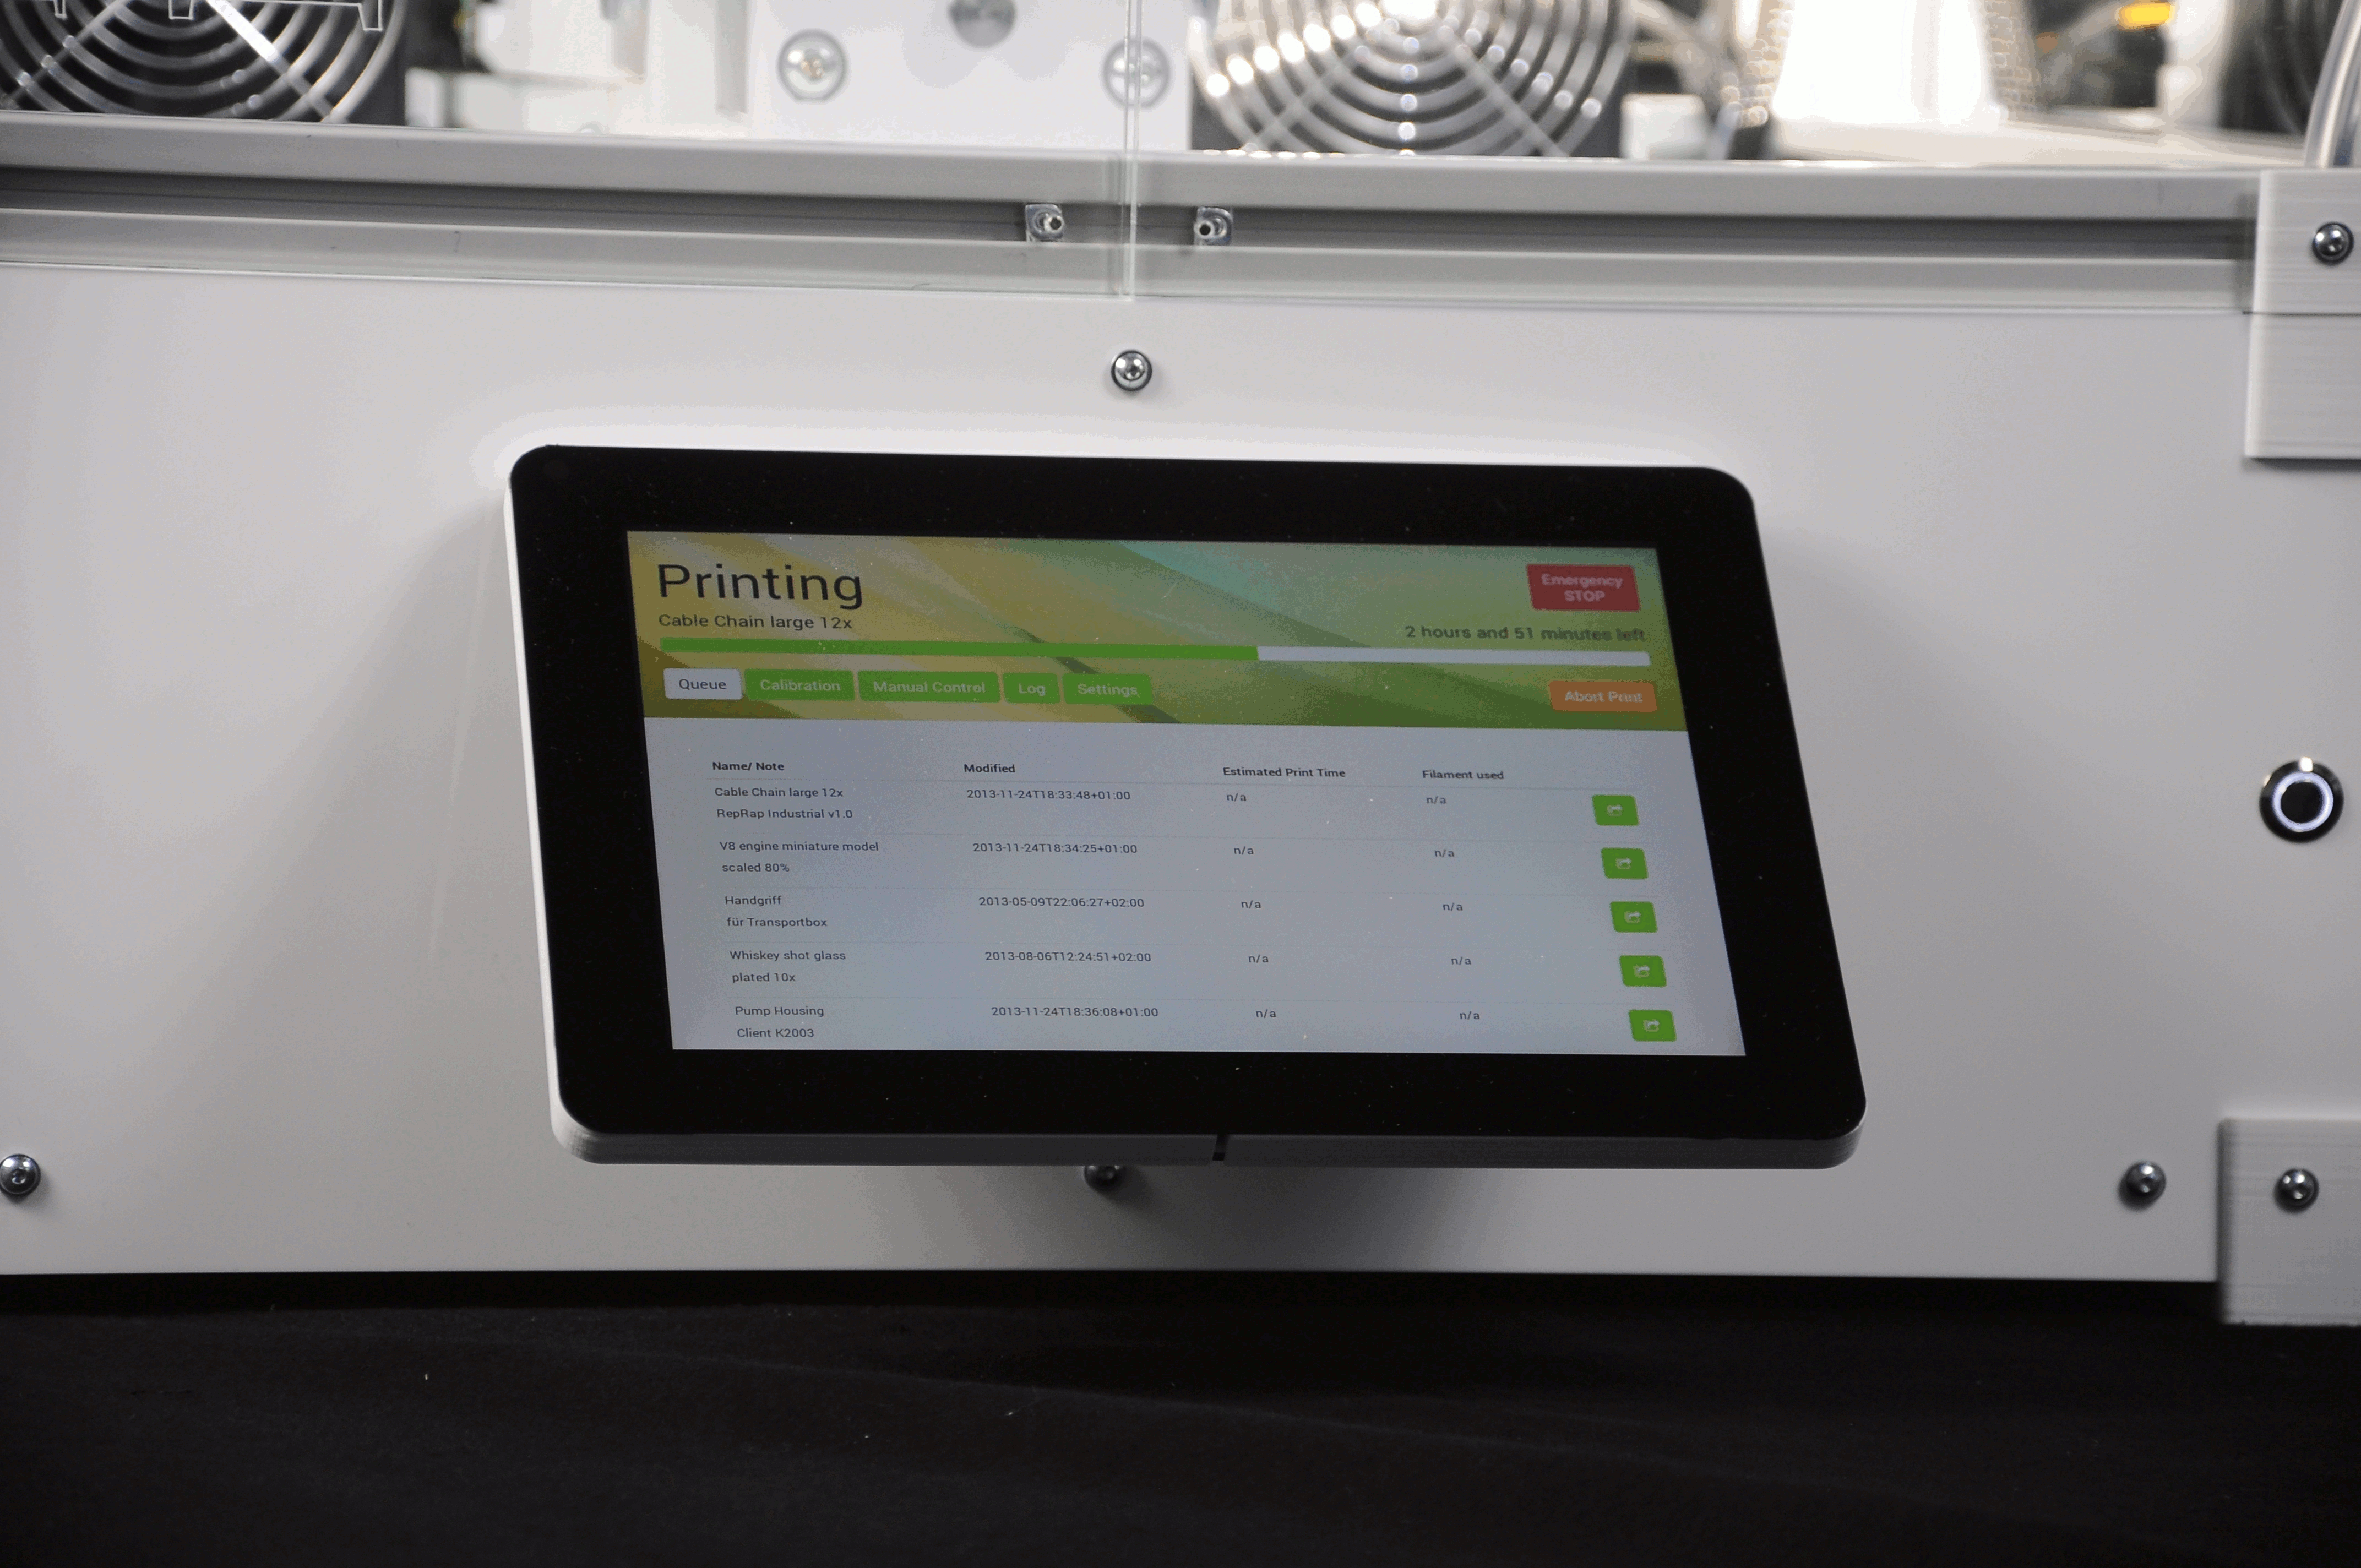
\includegraphics[width=.7\linewidth]{./img/touchscreen.png}
  \caption{The high-resolution 10\textquotedbl -TFT touchscreen mounted at the front 
           panel enables direct operation of the HT500.3.}
\end{figure}


This manual describes the initial commissioning of the 3D Printer after installation, the operation via the RepRapOnRails operating software and the all manual operating tasks that must be performed during normal day-today use.

\subsection{Starting the 3D Printer}

There are two possible states from which to start the 3D Printer: “switched off” and in “standby”. Either way starting the 3D Printer is a one-button-only procedure. After the boot sequence the operating screen starts with the Print screen in IDLE mode. 


\subsubsection{Switching on}

If the 3D Printer is switched off via the main switch at the rear cover 
(position \emph{<0>)} toggle the switch to \emph{<I>} (ON).
The 3D Printer will boot automatically.
It may take a few minutes until the touchscreen has fully loaded the operating screen - wait patiently without interfering.
The first screen will be the \emph{Print} screen with the (empty) print-job queue and the top-left status message displaying \emph{Idle}. 

\begin{figure}[H]
  \centering
  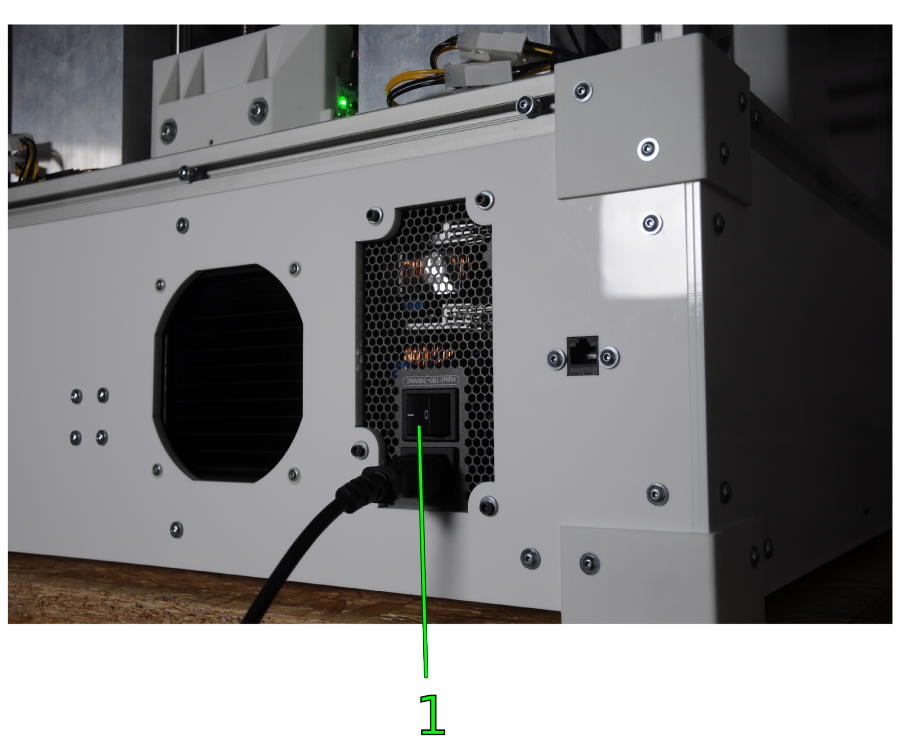
\includegraphics[width=.7\linewidth]{./img/opm_powerbutton.png}
  \caption{Powering up the 3D Printer.}
\end{figure}


\subsubsection{Waking from standby}

If the 3D Printer has been shut down via the touchscreen and set into standby mode (see section Print screen), press the wake button at the front cover. The light ring of the button lights up and the 3D Printer boots automatically.

\begin{figure}[H]
  \centering
  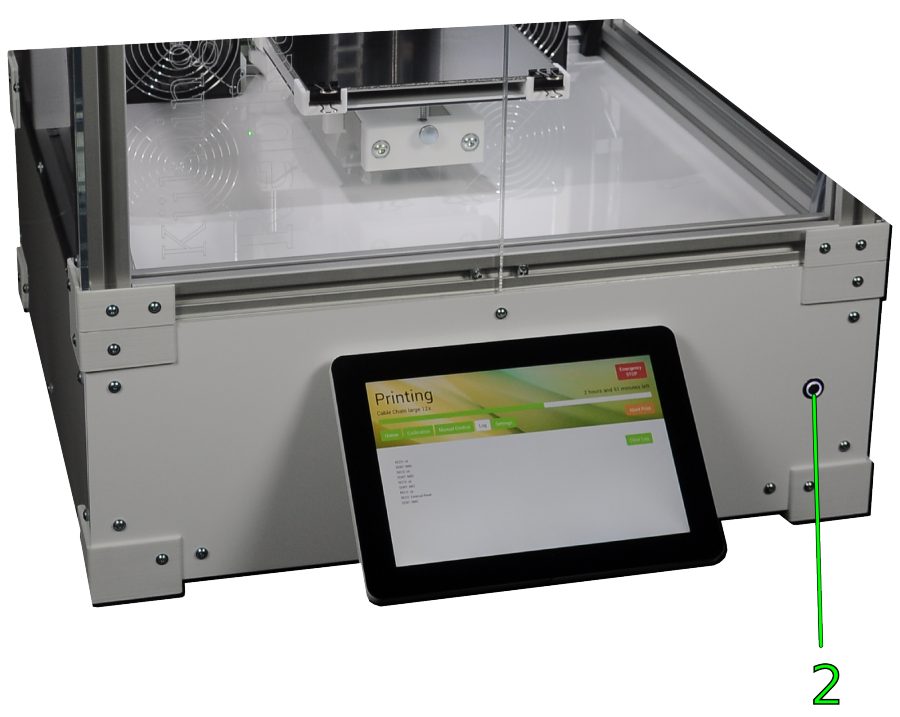
\includegraphics[width=.7\linewidth]{./img/opm_wakebutton.png}
  \caption{Waking the 3D Printer from standby.}
\end{figure}


\subsection{Graphical User Interface (GUI)}

\begin{figure}[H]
  \centering
  
\includegraphics[width=.7\linewidth]{./img/gui_menues_v110.png}
  \caption{Menu selection of the RepRapOnRails operating software.}
\end{figure}

The start-up \emph{Print} screen provides all basic operating functions.
The \emph{Configuration} menu enables the operator to preselect temperature profiles for the extruders and the print bed and build chamber more directly which simplifies preheating and priming according to current needs.
\emph{Setup} offers the operating wizards for guided day-to-day functions.
More advanced features such as program-independent operation of the axes can be found on the \emph{Expert control} screen which also provides direct setting of the extruder temperatures and test extrusion.
The \emph{Log} menu contains the history of machine code input and output as well as the keyboard for direct input of operating instructions.
The following paragraphs provide detailed information of the software's operating screens and explain the specific functions.
Additional information for the preparation of print jobs can be found in Tips and tricks and the manual of the slicing software. 


\subsubsection{[Print] screen}

 After starting the HT500.3 the \emph{Print} screen will appear as the start-up screen. Here you activate the 3D Printer and start the print jobs previously uploaded to the queue via the web interface.

\begin{figure}[H]
  \centering
  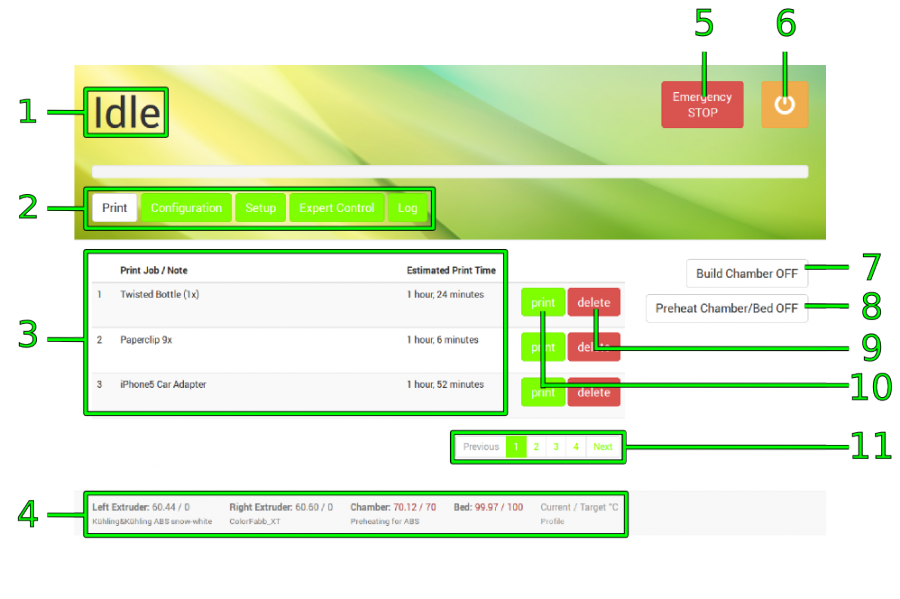
\includegraphics[width=.7\linewidth]{./img/gui_printtabnumber_v110.png}
  \caption{Print screen (descriptions may apply to other screens as well if not 
           explicitly given there)}
\end{figure}

\begin{table}[H]
  \centering
  \begin{tabulary}{\textwidth}{ L L L }
    \toprule
    No.   
      & Description   
        & Content/Function \\
    \midrule
    1   
      & Status message  
        & Idle: apparatus is waiting for next user input \newline
          Printing: apparatus is busy printing  \\
   2  
      & Menu selection  
        & Select the operating menu and mode: 
          Print represents the main production mode \newline
          Configuration allows choosing material based temperature profiles for each extruder and bed/chamber  \newline
          Setup provides wizards for different preset operating procedures
          Expert Control provides access to motors and direct temperature control \newline
          Log represents the communication history of machine\\
   3  
      & Queue   
        & List of uploaded print jobs sorted by time/date (oldest first); estimated 
          time required for printing the respective job. \\
   4  
      & Temperature/profile overview  
        & Displays current and set temperature of each extruder, print bed and build 
          chamber as well as the selected material profiles (see Configuration). Temperatures colored red are set and currently being actuated. \\
   5  
      & [Emergency STOP] button   
        & see also \newline
          $\rightarrow$ Emergency stop \newline
          $\rightarrow$ Safety information in the Manual \\
   6  
      & [Shut-down] button  
        & Tap to shut down the 3D Printer properly. \\
   7  
      & [Build Chamber ON/OFF] button   
        & Tap to activate/deactivate drives and heaters after start-up. \\
    \bottomrule
  \end{tabulary}
\end{table}


\paragraph{Starting print jobs}

Tap the [print] button next to a print job in the queue to start the print job. You will be asked to confirm that all preparations for the print job have been performed. Tap [OK, Start Print] to definitely begin printing or [Cancel] to return to the queue. 

\begin{figure}[H]
  \centering
  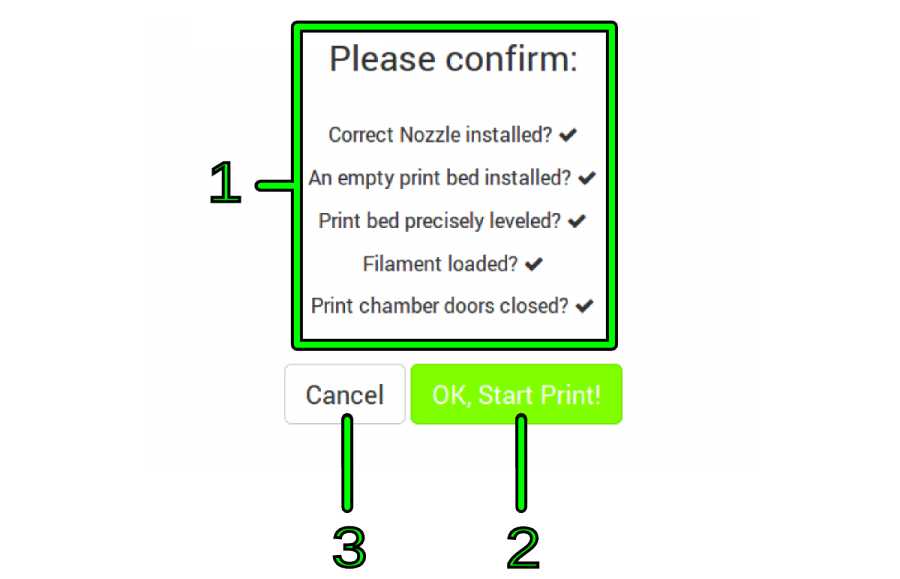
\includegraphics[width=.7\linewidth]{./img/om_confirm_pj.png}
  \caption{“Ready to print?” query}
\end{figure}

\begin{table}[H]
  \centering
  \begin{tabulary}{\textwidth}{ L L L }
    \toprule
    No.   
      & Description   
        & Content/Function \\
    \midrule
    1   
      & Checklist   
        & Please make sure that all displayed requirements have been met before 
          proceeding. \\
    2   
      & [OK, Start Print] button  
        & If all preparations have been made, tap to proceed. \\
    3   
      & [Cancel] button   
        & Tap to abort if any requirements has not been met. \\
    \bottomrule
  \end{tabulary}
\end{table}

After confirmation the HT50.3 starts processing the print job and the status message changes to \emph{Printing}. All other menus are deactivated during a print. The print job name, the current progress, and the estimated remaining time are displayed and the 
[Abort Print] button is active.

\begin{figure}[H]
  \centering
  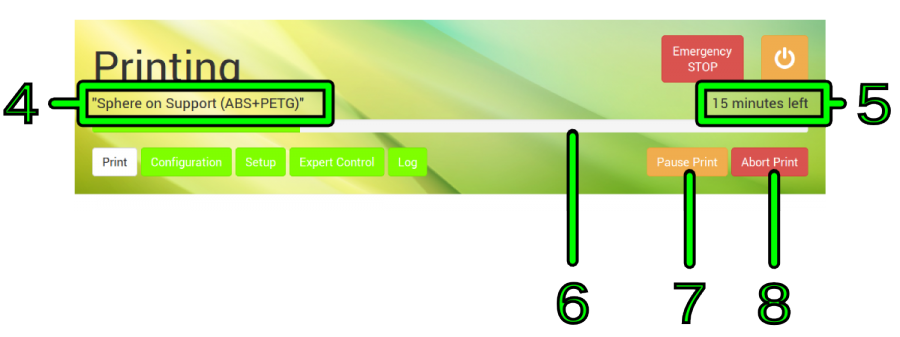
\includegraphics[width=.7\linewidth]{./img/om_currently_printing.png}
  \caption{Print status screen (top half only).}
\end{figure}

\begin{table}[H]
  \centering
  \begin{tabulary}{\textwidth}{ L L L }
    \toprule
    No.   
      & Description   
        & Content/Function \\
    \midrule
    4   
      & Print job name  
        & The name of the slicing file uploaded to the queue. \\
    5   
      & Countdown   
        & Displays the estimated remaining time (calculated from the G-code). \\
    6   
      & Progress bar  
        & Indicates the progress of the print job graphically. \\
    7   
      & [Pause/Resume Print] button   
        & Allows interrupting a print job for interference 
          and subsequent resumption.  \\
    8   
      & [Abort Print] button  
        & Tap to abort a print job. \\
    \bottomrule
  \end{tabulary}
\end{table}


\paragraph{Pause function}

The pause function was built in for the case that a print job needs to be interrupted and later resumed for other reasons than “out-of-filament” (see below).

\begin{figure}[H]
  \centering
  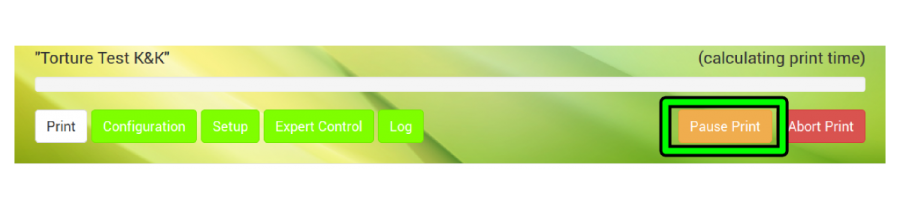
\includegraphics[width=.7\linewidth]{./img/om_pause_print.png}
  \caption{Interrupting the print with the pause function.}
\end{figure}

After tapping the [Pause Print] button, the printer keeps printing until the cache is empty. This may take a few minutes, according to the complexity of the current g-code. Afterwards, the print bed is lowered into its home position, the extruders are turned off and the print head moves to the maintenance position.
Now you have access to the Expert Controls and some of the Setup functions to adjust whatever might be necessary.

\begin{figure}[H]
  \centering
  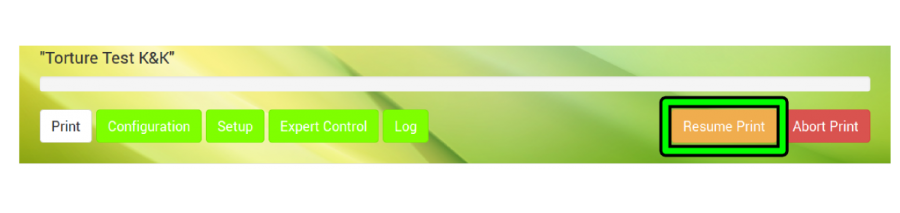
\includegraphics[width=.7\linewidth]{./img/om_resume_print.png}
  \caption{Continuing the print after pause.}
\end{figure}

To continue printing tap [Resume Print] (replaced [Pause Print]). Print bed and extruder head move to their last position and after re-heating the extruders the print continues. 

\paragraph{Finishing a print job}

There are two ways to finish a print job: automatic finish after completion or abortion by the operator.
After regularly completing a print job all axes are moved to their home position and the extruder heating resistors are switched off.
If you need to abort a print job because the outcome does not meet expectations for example or mechanical problems appear during the print, tap the [Abort Print] button. The system will then print the last G-code information from cache and move the print table and the extruder head to their home positions afterwards.
Either way, the 3D Printer returns to idle mode and displays a status message and a request how you wish to continue. Simply tap the respective button on the screen to proceed.
After standstill of all drives you can remove the print bed and take off the model. 

\begin{figure}[H]
  \centering
  
\includegraphics[width=.7\linewidth]{./img/gui_finishedprinting_v110.png}
  \caption{Print job finished.}
\end{figure}

\begin{table}[H]
  \centering
  \begin{tabulary}{\textwidth}{ L L L }
    \toprule
    No.   
      & Description   
        & Content/Function  \\
    \midrule
    9   
      & [Keep in Queue]   
        & Returns to the Print menu. \\
    10  
      & [Print Again]   
        & Immediately restarts the current print job. \\
    11  
      & [Delete Printjob]   
        & Deletes the finished print job from the queue without confirmation and 
          returns to the Print menu. \\
    \bottomrule
  \end{tabulary}
\end{table}


\paragraph{Switching off the 3D Printer}

\begin{notice}
  Switching off the 3D Printer via the power button without turning it into standby may cause damage of the heating elements and neighboring components due to residual heat.
  The cool-down performed during shut-down ensures that the fans are only switched off after the heating elements could shed all residual heat.
\end{notice}

\begin{figure}[H]
  \centering
  
\includegraphics[width=.7\linewidth]{./img/om_power_off_button.png}
  \caption{Always use this button for regular shutdown.}
\end{figure}

For switching the HT500.3 into standby tap the shut-down button. The system will then perform the cool-down sequence for safety reasons before deactivating the preheating and the build chamber.

The 3D Printer is in standby mode when:

\begin{itemize}
  \item the screen turns black,
  \item the illuminated ring of the wake button dims,
  \item the build chamber lighting switches off.
\end{itemize}

To wake the machine from standby see $\rightarrow$ emph{Starting the 3D Printer}.. 

For completely shutting down the 3D Printer, perform the procedure described above and set the main switch at the rear cover to \emph{<0>} (OFF) afterwards. The 3D Printer is now powered off.
To reactivate the 3D Printer see $\rightarrow$ emph{Starting the 3D Printer}. 

\begin{info}
  For day-to-day use, the power supply should stay connected to mains power (main switch in position \emph{<I>} (ON). 
\end{info}


\paragraph{Emergency stop}

\begin{notice}
  The emergency stop function does not provide a cool down sequence. \emph{Do not} use the emergency stop button to abort current print jobs, as this may lead to damage of the 3D Printer due to uncontrolled heat accumulation. \emph{Do not} use the main switch as an emergency stop button. You risk loosing or corrupting data. 
\end{notice}

\begin{figure}[H]
  \centering
  
\includegraphics[width=.7\linewidth]{./img/gui_v110_emergencystoptriggered.png}
  \caption{Status display after triggering the emergency stop. The 3D Printer 
           returns to IDLE state after a short time. The emergency stop is written into the log-file. }
\end{figure}

When the emergency stop is triggered:

\begin{itemize}    
  \item The machine controller board is reset, all movement of the axes stops, lights, 
        heaters and fans are turned off. The status indicator displays
        \emph{Emergency Stop}!.
  \item After a few seconds the machine controller returns to \emph{Idle} state.
\end{itemize}

The 3D Printer now is in a safe state for troubleshooting.
For repairing \emph{any defects of the electronic equipment or major mechanical damages shut down the 3D Printer completely:}

\begin{itemize}
  \item Shut down the 3D Printer by tapping the \emph{[Shutdown]} button and switching
        off the main switch (\emph{<0>} position) after the shutdown procedure has been finished.
\end{itemize}

\begin{notice}
   Before restarting or reactivating the 3D Printer:
   \begin{itemize}
     \item Make sure that the axes are in no collision position.
     \item Make sure that the reason for the emergency stop has been detected and 
           fixed, before resuming production.
   \end{itemize}
\end{notice}

 After troubleshooting or if the reason for the emergency stop was minor and you want to continue production:

\begin{itemize}
  \item Remove the print bed from the build chamber and replace or clean it before 
        further use.
  \item Restart the 3D Printer (if necessary).
  \item Open the Print screen.
  \item Switch on the build chamber. The 3D Printer will run the homing routine.
  \item You can now resume normal operation.
\end{itemize}


\subsubsection{[Configuration] screen}

 The \emph{Configuration} menu enables you to preselect material-specific temperature profiles for each extruder and, in combination, the print bed/build chamber. The latter is important to make preheating and leveling precise with regard to different material settings. The according profiles can be set up at the web interface setup menu.

\begin{figure}[H]
  \centering
  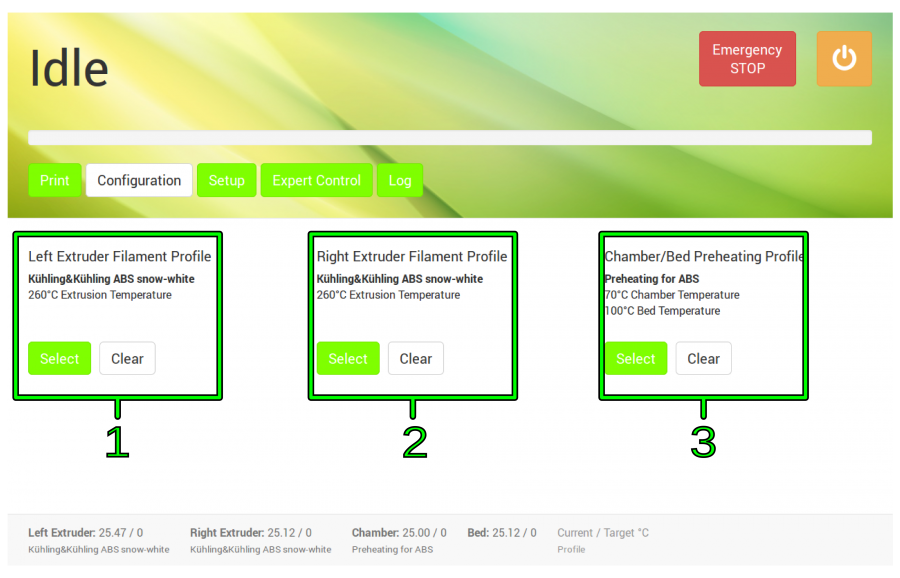
\includegraphics[width=.7\linewidth]{./img/gui_configmenu_1_v110.png}
  \caption{GUI Configuration screen with temperature profile selection}
\end{figure}

\begin{table}[H]
  \centering
  \begin{tabulary}{\textwidth}{ L L L }
    \toprule
    No.   
      & Description   
        & Content/Function  \\
    \midrule
    1   
      & Left extruder profile selection   
        & The currently selected profile is displayed.
          Tap \emph{[Select]} to open the list of available filament profiles or [Clear] to delete the active profile. \\
    2   
      & Right extruder profile selection
        & same as above \\
    3   
      & Bed/chamber profile selection   
        & The currently selected profile is displayed. 
          Tap [Select] to open the list of available filament profiles or [Clear] to delete the active profile.
          After selection of a profile, deactivate the preheating function in the Print menu (touch button no. 8) and activate it by tapping the button again to apply the settings.  \\
    \bottomrule
  \end{tabulary}
\end{table}

\begin{figure}[H]
  \centering
  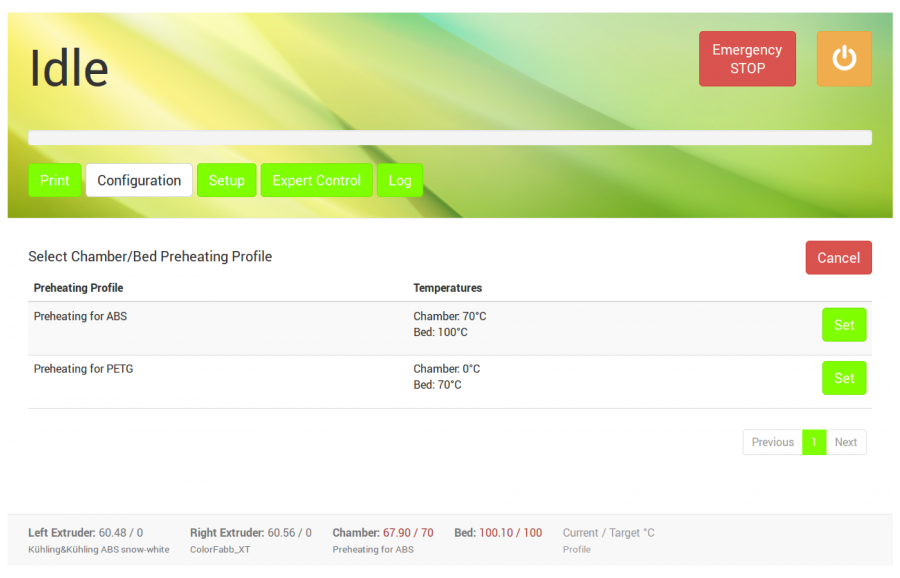
\includegraphics[width=.7\linewidth]{./img/gui_configmenu_2_v110.png}
  \caption{The list of chamber/bed temperature profiles of the configuration menu. More 
           profiles can be added via the web-interface.}
\end{figure}

After opening the list, tap [Set] to choose a profile for the selected component. The profile is set and the screen returns to the prior menu.
To activate the selected profile open the Print screen and first deactivate, then re-activate the chamber/bed preheating. 

\begin{figure}[H]
  \centering
  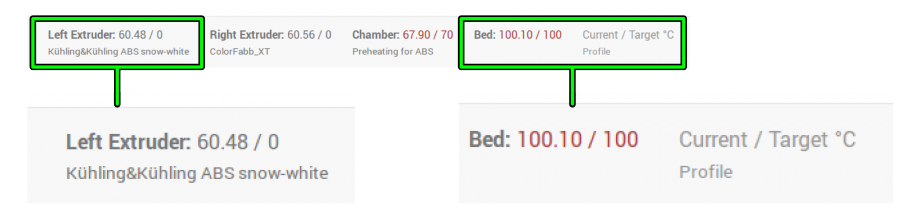
\includegraphics[width=.7\linewidth]{./img/gui_configmenu_3_v110.png}
  \caption{The selected profiles are displayed in the footer of the GUI on every 
           screen.}
\end{figure}

The selected profiles are displayed in the footer of every screen in the order 
\emph{Current} and \emph{Target} (= set) temperature. While aiming for a target temperature, both values are highlighted red. When displayed gray, the temperature value is either not set or currently not triggered.
If no filament profile is activated for an extruder, the default temperature is 
180\degree C. 

\begin{info}
  Observe that the temperature shown in the footer is measured at the hot end heater and may be 5 - 10\degree C lower at the nozzle tip.
  See section \emph{Extrusion temperature} in the knowledgebase for information on finding the suitable extrusion temperature.
\end{info}


\subsubsection{[Setup] screen}

The \emph{Setup} menu displays walkthrough instructions (wizards) for different operations needed during daily operation, initial commissioning, servicing and troubleshooting. If you choose one of the wizards, a step-by-step guide will provide all necessary information for completing the respective task.
This screen also provides system information and the web address needed to connect to the 3D Printer via the network. 

\begin{figure}[H]
  \centering
  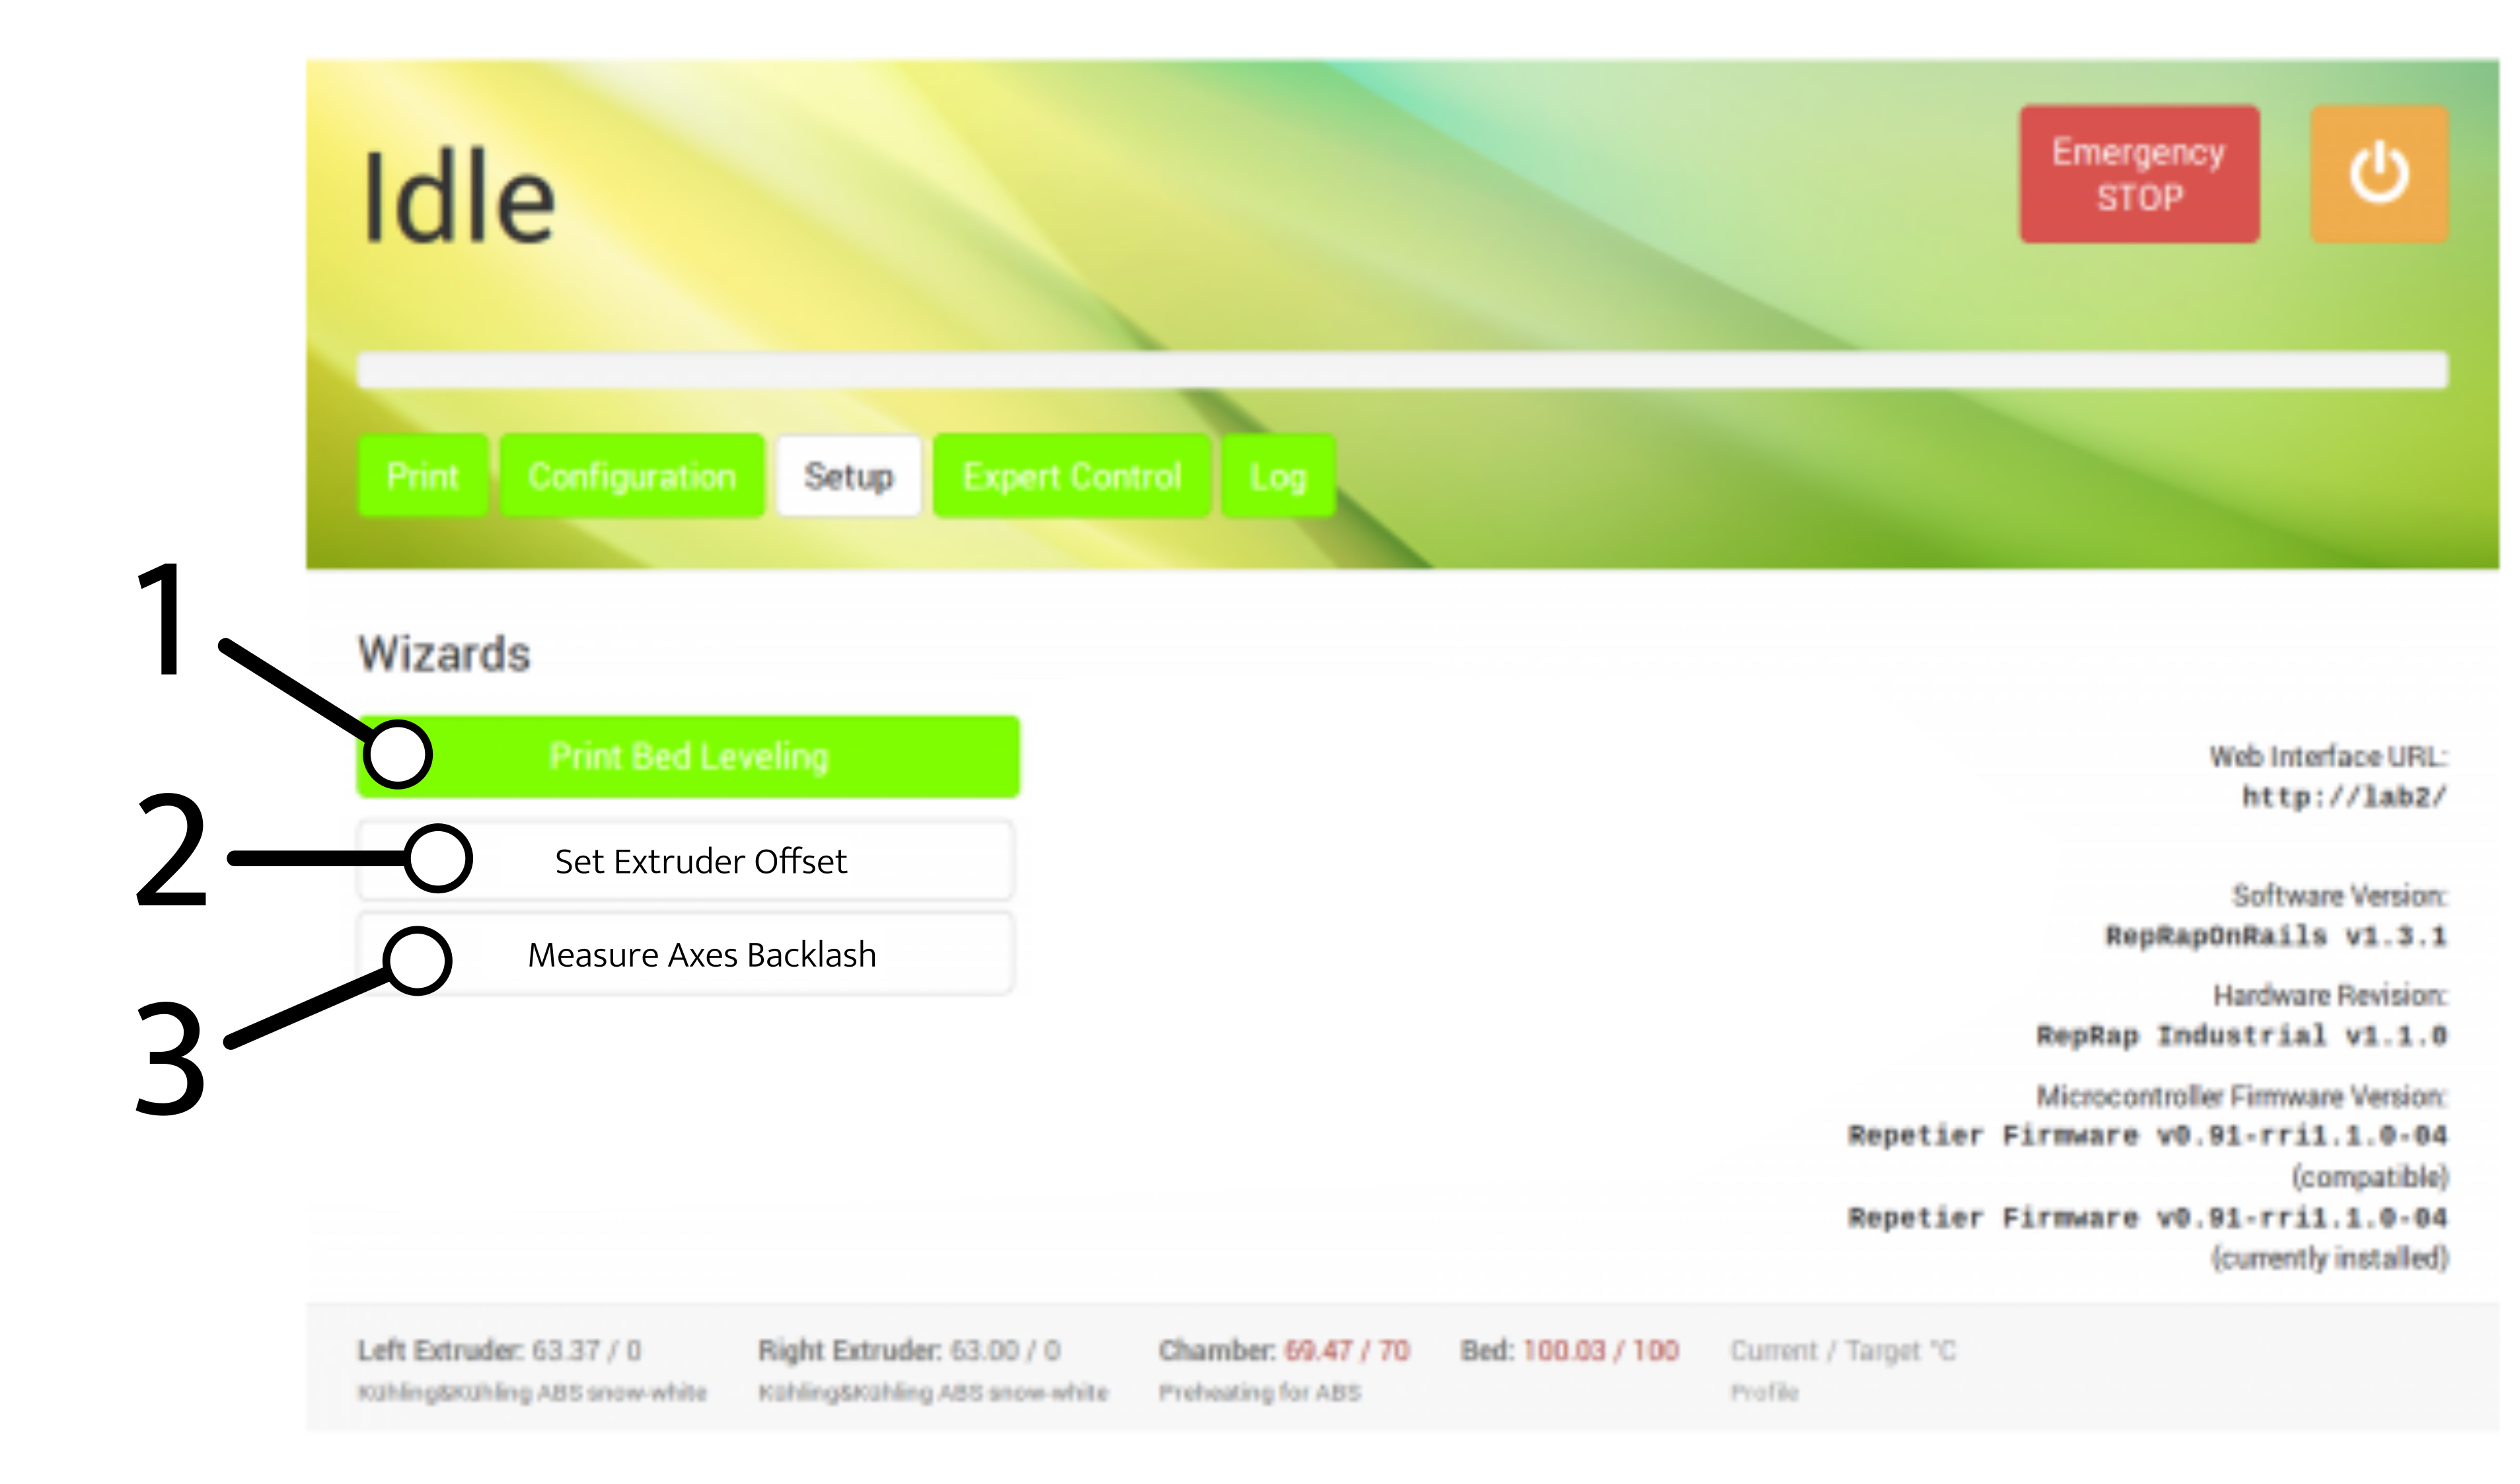
\includegraphics[width=.7\linewidth]{./img/gui_setup_wizards.png}
  \caption{Wizard selection on the setup screen. Beginning with ReRapOnRails v1.3.0, 
           the nozzle change wizard has been replaced by the backlash calibration wizard.}
\end{figure}

\begin{table}[H]
  \centering
  \begin{tabulary}{\textwidth}{ L L L }
    \toprule
    No.   
      & Description   
         & Content/Function \\
    \midrule
    1
      & Print Bed Leveling
         & Ensures that print bed and nozzle tip are evenly distanced at every point of the surface.\\
    2
      & Set Extruder Offset
         & Adjust the offset between left and right nozzle for precise alignment in dual-extruder prints.\\
    3
      & Measure Axes Backlash
         & Automatic measurement routine to inspect axes backlash in the drive system. Used for diagnosis 
           in technical support \\
    \bottomrule
  \end{tabulary}
\end{table}

\begin{figure}[H]
  \centering
  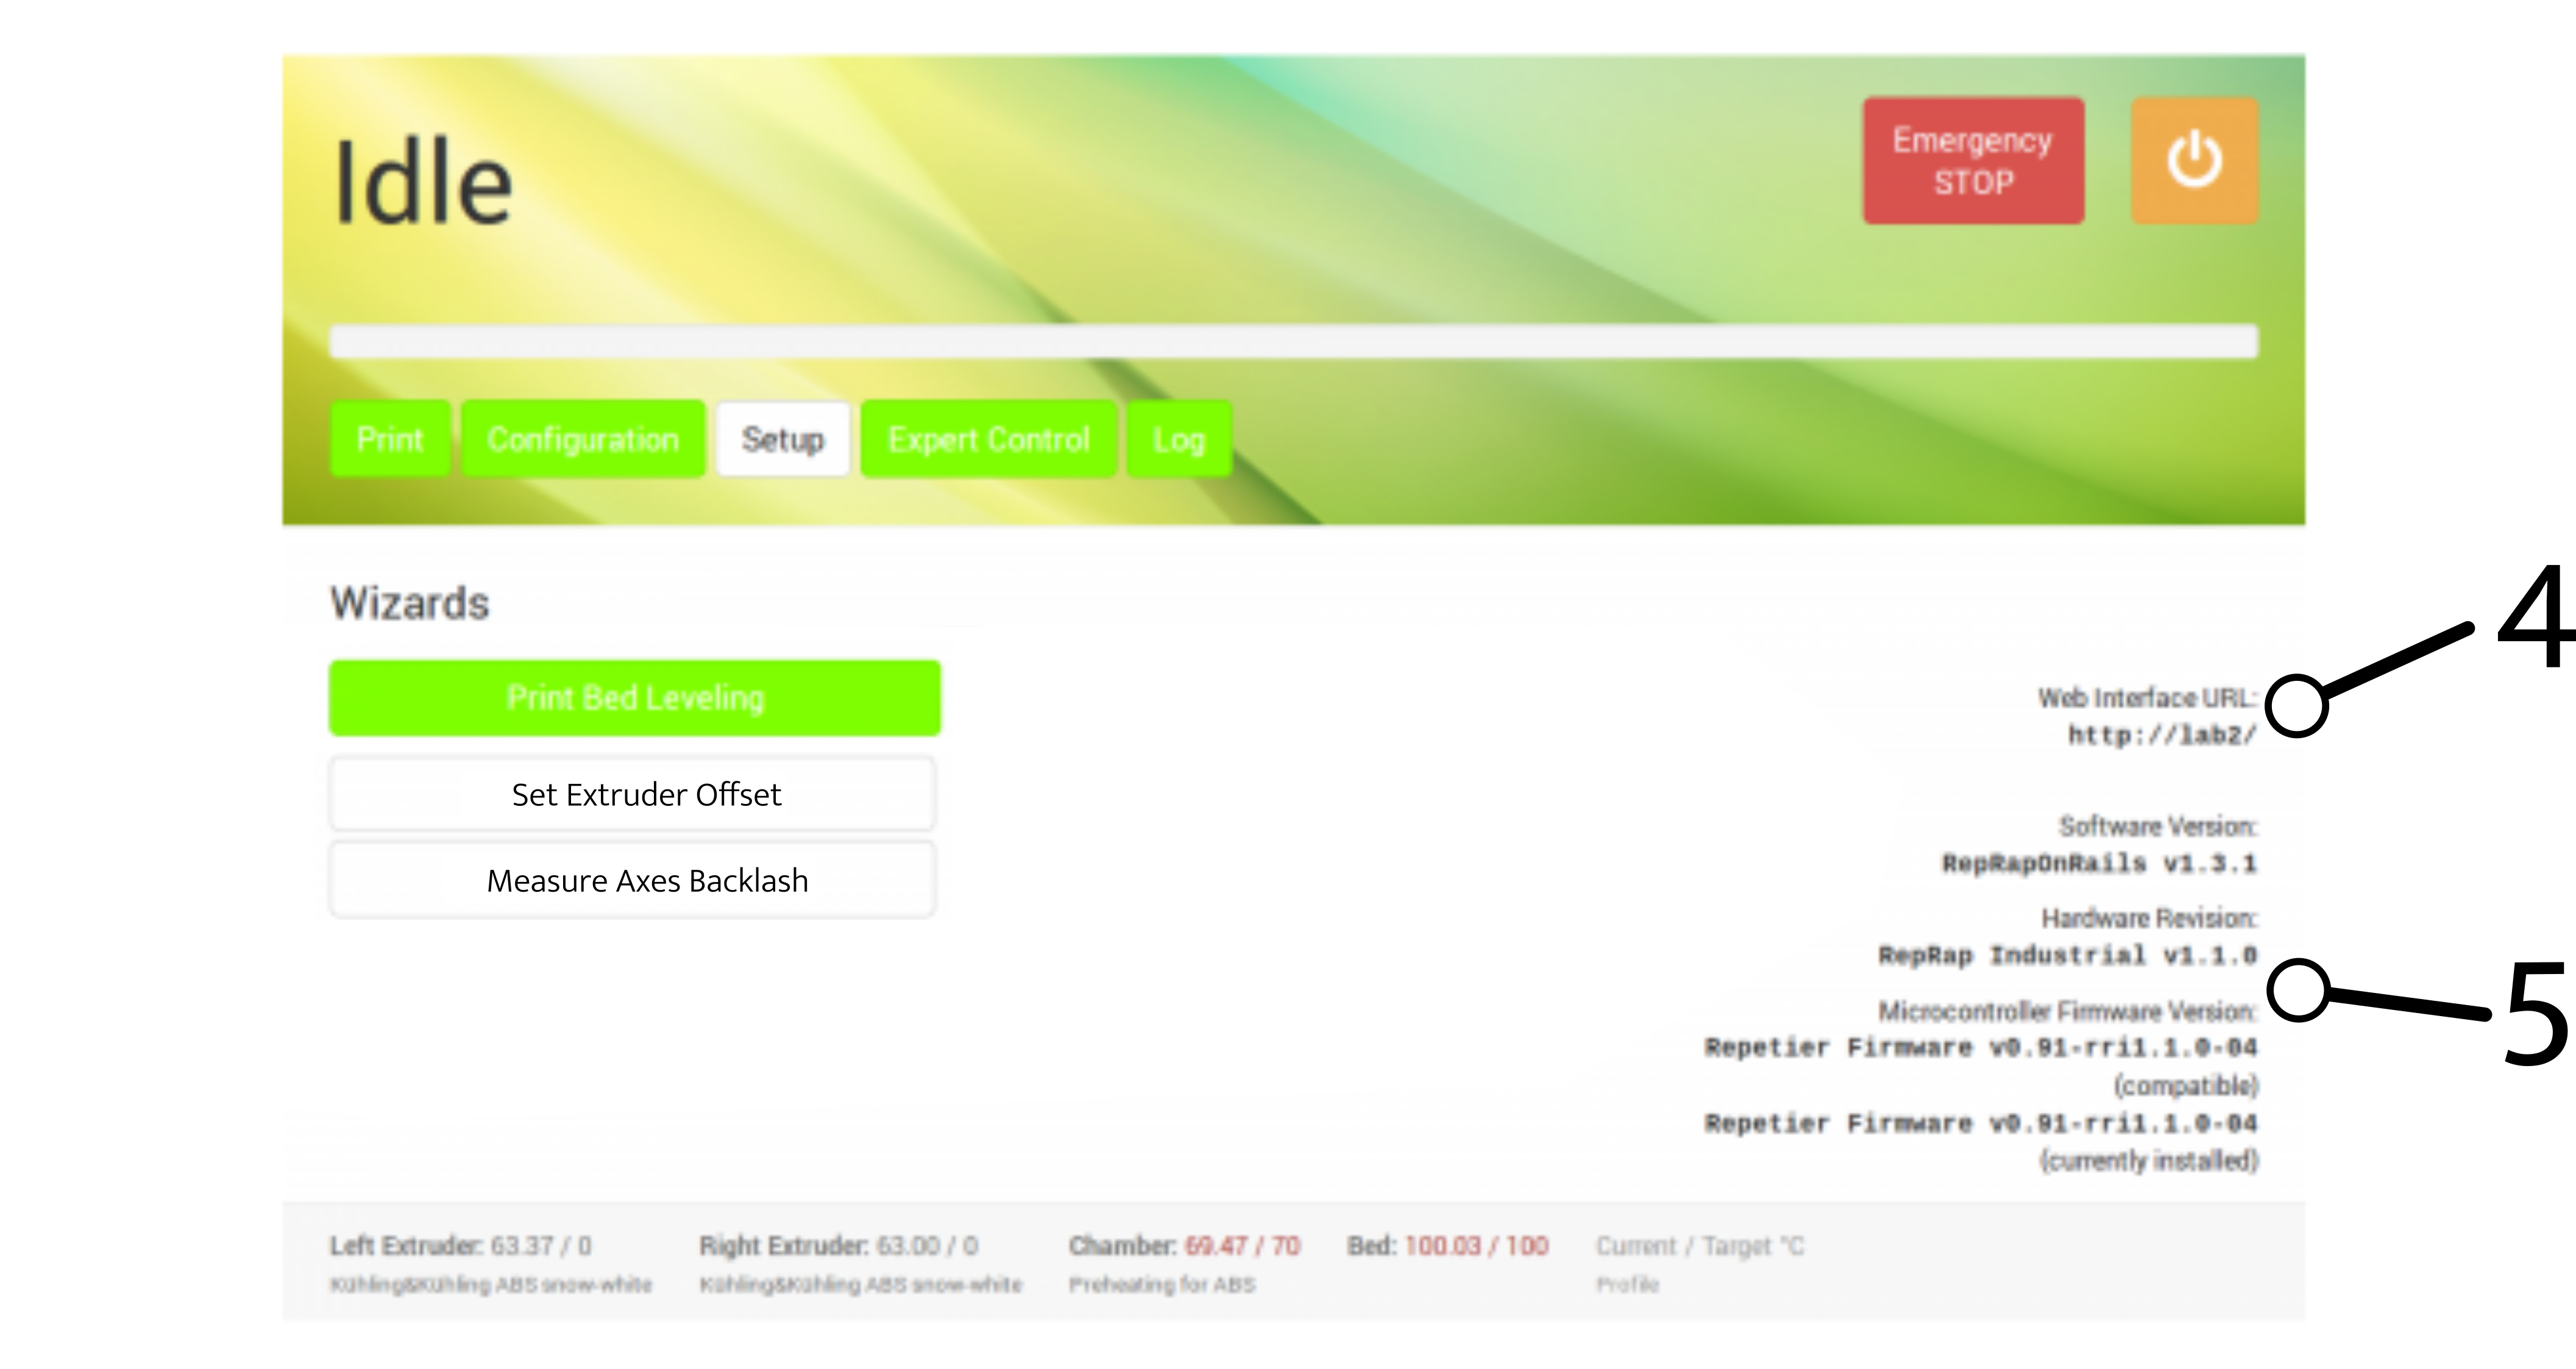
\includegraphics[width=.7\linewidth]{./img/gui_setup_info.png}
\end{figure}

\begin{table}[H]
  \centering
  \begin{tabulary}{\textwidth}{ L L L }
    \toprule
    No.   
      & Description   
        & Content/Function  \\
    \midrule
    4   
      & Web Interface URL 
        & Needed to connect to your HT500.3 via the network\\
    5  
      & Version numbers 
        & The valid version numbers of your HT500.3's hardware, the installed 
          RepRapOnRails software and the microcontroller firmware for your information. Please provide these numbers for identification in case of service requests.\\
    \bottomrule
  \end{tabulary}
\end{table}

\subsubsection{[Expert Control] screen}

\begin{notice}
  The Expert Control menu should be used by skilled operators only. Persons unfamiliar with the 3D Printer must not use the functions provided here.
  The positions of the extruder head and the print table are not compared during manual operation. Incautious operation may lead to massive damage of the extruder head and the print bed.
  Be careful not to crash the print table and the extruder head. 
\end{notice}

The [Expert Control] screen provides ability to manually move the X/Y/Z axes of the 3D printer as well as manually setting extruder temperature and priming (eg. for loading/unloading filament)

\begin{figure}[H]
  \centering
  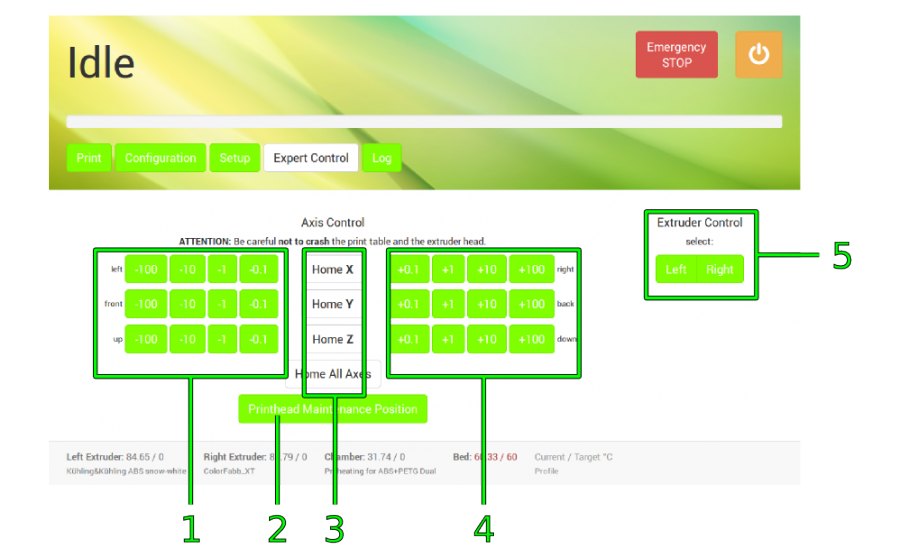
\includegraphics[width=.7\linewidth]{./img/gui_expertmenu_1_v110.png}
  \caption{Expert Control screen}
\end{figure}

\begin{table}[H]
  \centering
  \begin{tabulary}{\textwidth}{ L L L }
    \toprule
    No.   
      & Description   
        & Content/Function \\
    \midrule
    1   
      & Drive control - negative direction  
        & Moves every axis individually once for every tap in negative direction, 
          according to the selected step width. \\
    2   
      & [Printhead Maintenance Position]  
        & Tap to move the extruder head into a preset position in the upper center 
          of the build chamber directly in front of the doors where it is easily accessible for maintenance purposes. \\
    3   
      & Homing buttons  
        & Tap to separately or simultaneously move the axes to their starting 
          positions. \\
    4   
      & Drive control - positive direction  
        & Moves every axis individually once for every tap in positive direction, 
          according to the selected step width. \\
    5   
      & Extruder temperature control  
        & Enables directly setting the temperature and extruding filament for one 
          extruder at a time.  \\
    \bottomrule
  \end{tabulary}
\end{table}


\subsubsection{[Log] screen}

All actions of the machine controller is stored and displayed on the log screen. Print job statuses are stored also.
Direct G-code programming can be effected via the G-code input field. 

\begin{figure}[H]
  \centering
  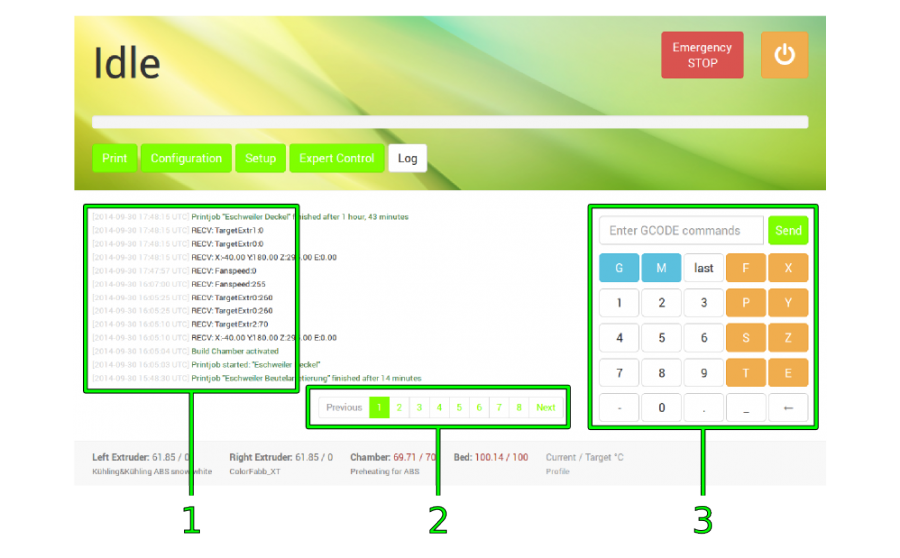
\includegraphics[width=.7\linewidth]{./img/gui_logmenu_v110.png}
  \caption{The log screen provides additional information about sent and received 
           G-code commands and the possibility of directly influencing the 3D Printer via G-code command input.}
\end{figure}

\begin{table}[H]
  \centering
  \begin{threeparttable}
    \begin{tabulary}{\textwidth}{ L L L }
      \toprule
      No.   
        & Description   
          & Content/Function  \\
      \midrule
      1   
        & History list  
          & communication history sorted top down by date and time \tnote[1] \newline
            SENT: RepRapOnRails host to machine controller\newline
            RECV: machine controller to RepRapOnRails host\\
      2   
        & Browse buttons  
          & Use [Previous], [Next] and [page number] to browse the history.  \\
      3   
        & G-code input field  
          & Enter G-code lines here and [Send] them.  \\
      \bottomrule
    \end{tabulary}
    \begin{tablenotes}\footnotesize
      \item[1] The time is stated in universal time coordinated (UTC) notation so do 
             not wonder if does not match your local time.
    \end{tablenotes}
  \end{threeparttable}
\end{table}
 
\begin{notice}
  The G-code input field is an advanced feature and requires sound knowledge of GCODE programming. Inappropriate use may cause damage to the 3D Printer.
\end{notice}


\subsection{The web interface}

The web interface provides the communication between your PC and the 3D Printer. Uploading print job GCODES to the 3D Printer and creating temperature profiles are the main functions.
You can also check system's information and settings, install firmware updates and download the LOG-file for troubleshooting purposes.

To open the web interface enter the web interface URL into the address line of your internet browser. You can find the web interface URL on the Setup screen of the GUI.

\subsubsection{First Steps}

\begin{figure}[H]
  \centering
  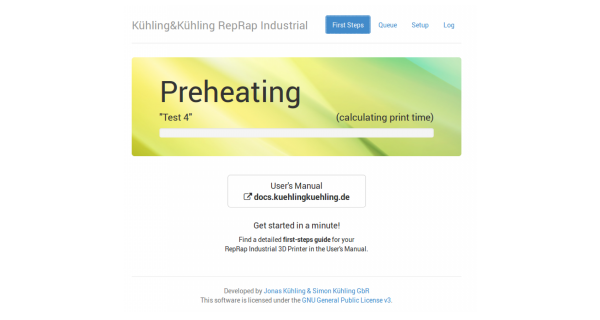
\includegraphics[width=.7\linewidth]{./img/wi_firststeps_printstarted.png}
  \caption{First Steps screen of the web interface.}
\end{figure}

\subsubsection{Queue}

Print jobs are managed via the Queue. Here you can upload GCODES, individaully name, edit, or delete them. 

\begin{figure}[H]
  \centering
  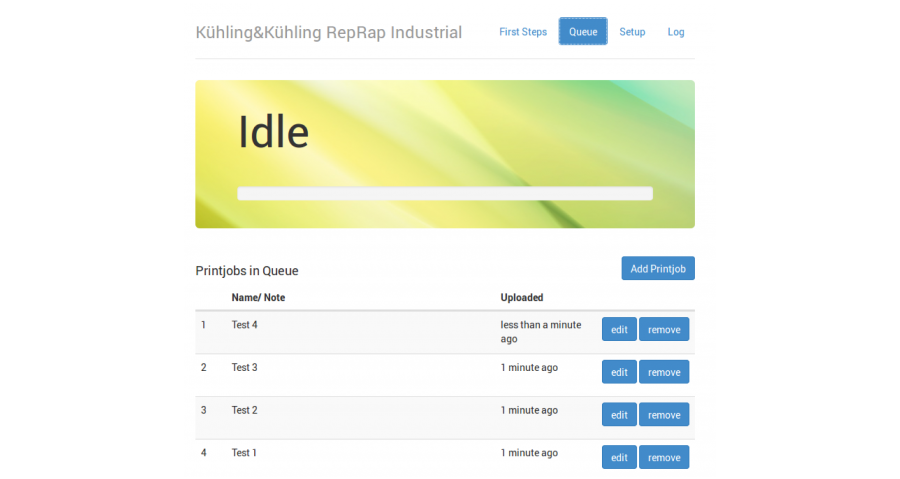
\includegraphics[width=.7\linewidth]{./img/wi_queue_1.png}
  \caption{The Queue contains list of uploaded print jobs in a top-down order with 
           the last upload first.}
\end{figure}

\begin{figure}[H]
  \centering
  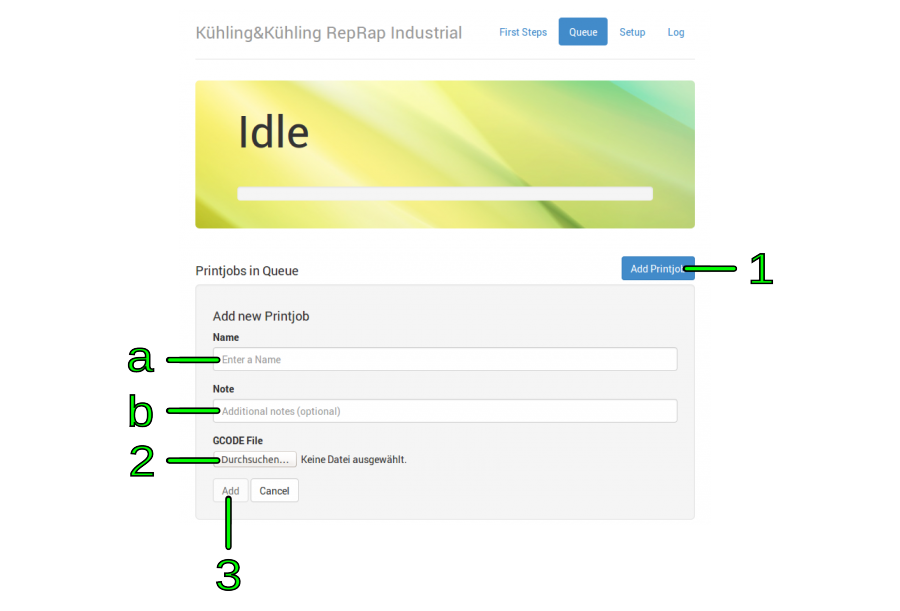
\includegraphics[width=.7\linewidth]{./img/wi_queue_2.png}
  \caption{Uploading print jobs to the Queue.}
\end{figure}

To create a print job:

\begin{enumerate}
  \item Click [Add Printjob].
    \begin{enumerate}
      \item Enter the identification (name or number or the like) of the print job in the text field \emph{Name}. This will be shown in the status field during the print job is conducted.
      \item If required, add additional information via the text field \emph{Note}.
    \end{enumerate}
  \item Click [Browse] to select a GCODE from the valid directory.
  \item Click [Add] to upload the selected file to the printer. The print job is 
        added to the list as the first entry.
        Click \emph{[Cancel]} to abort the procedure.
\end{enumerate}

The print job is now available for printing on your HT500.3 and can be selected directly for printing via the touchscreen controller on the 3D Printer.

\begin{figure}[H]
  \centering
  
\includegraphics[width=.7\linewidth]{./img/wi_queue_3.png}
  \caption{Editing or deleting print jobs from the web interface queue.}
\end{figure}

\begin{enumerate}
  \item To subsequently renaming print jobs or altering information 
        click on \emph{[edit]} and use the text fields.
  \item To delete a print job from the queue click on \emph{[remove]} and 
        acknowledge the query by clicking \emph{<OK>}.
\end{enumerate}


\subsubsection{Setup}

In the \emph{Setup} menu temperature profiles for materials and print bed/chamber can be managed, system information can be viewed, firmware updates can be conducted and, EEPROM-data can be set. 

\begin{figure}[H]
  \centering
  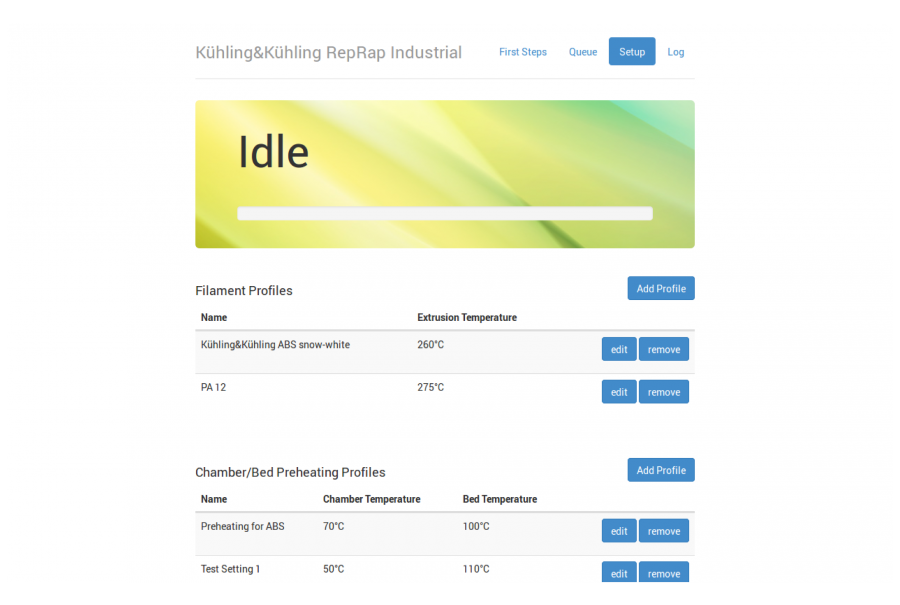
\includegraphics[width=.7\linewidth]{./img/wi_setup_1.png}
  \caption{Temperature profiles on the Setup screen of the web interface.}
\end{figure}

\begin{figure}[H]
  \centering
  
\includegraphics[width=.7\linewidth]{./img/wi_setup_11.png}
  \caption{System information that can also be found on the Setup screen of the GUI. 
           Please always provide these in case you contact the Technical Support. }
\end{figure}

\begin{figure}[H]
  \centering
  
\includegraphics[width=.7\linewidth]{./img/wi_setup_12.png}
  \caption{Installing a new machine controller firmware - which may only be done when 
           explicitely requested by Kühling\&Kühling - is done via the Setup menu. Find additional information in the Upgrade section.}
\end{figure}

\begin{figure}[H]
  \centering
  
\includegraphics[width=.7\linewidth]{./img/wi_setup_13.png}
  \caption{The EEPROM editor may only be used by experienced users or if explicitely 
           stated in this manual and strictly within the specified parameters. Its main purpose is helping the Technical Support during troubleshooting.}
\end{figure}


\paragraph{Creating temperature profiles}

During a print job all necessary temperature data are provided by the respective G-code. For priming the extruders outside a print job the temperature setting required for extruding a material is provided by the \emph{Filament profiles}.
Similarly, precise print bed leveling needs defined bed and chamber temperatures according to the printed material before a G-code is executed. These settings are provided by the \emph{Chamber/Bed Preheating Profiles}. 

\begin{figure}[H]
  \centering
  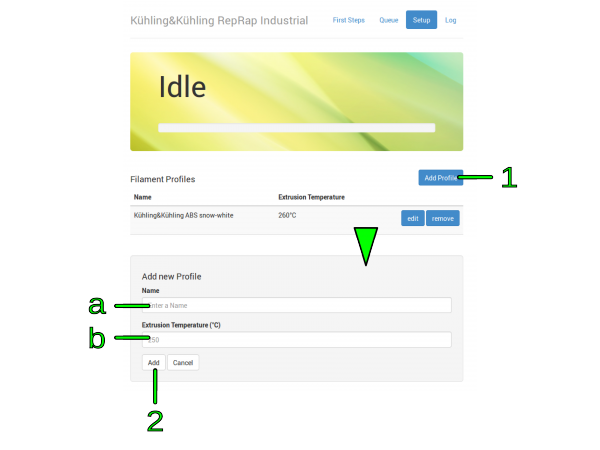
\includegraphics[width=.7\linewidth]{./img/wif_setup_addfilamentprofile.png}
  \caption{Filament profile setup via the web interface.}
\end{figure}

To create a filament profile open the web interface of your 3D Printer, choose the Setup menu and:

\begin{enumerate}
  \item Select Filament Profiles and click [Add Profile] to set material properties.
    \begin{enumerate}
      \item Enter the material Name in the according input field.
      \item Enter the Extrusion Temperature in \degree C in the according input field.
    \end{enumerate}
  \item Click [Add] or press <Enter> to save the settings. The new filament profile 
        is added to the list, newest at the bottom.
\end{enumerate}

\begin{itemize}
  \item To change the settings click [edit] and enter the new properties.
  \item To delete a profile click [remove] and confirm the safety query.
\end{itemize}

\begin{figure}[H]
  \centering
  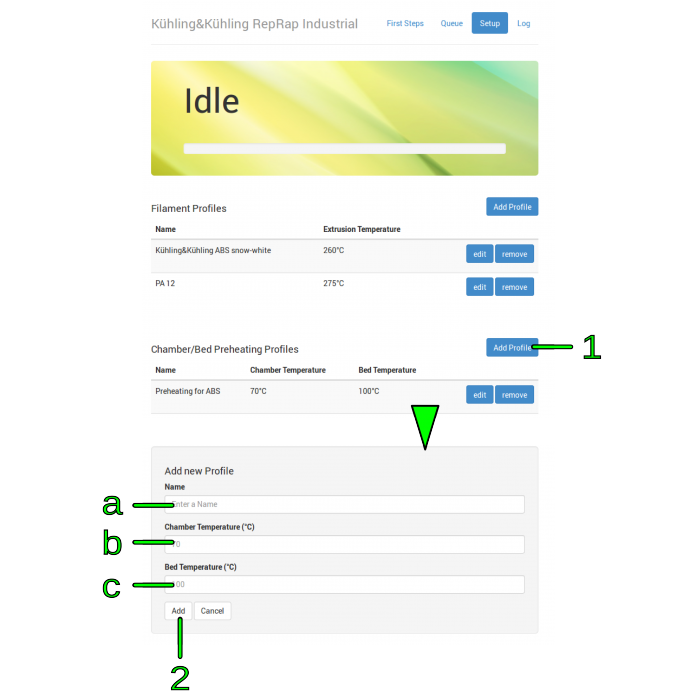
\includegraphics[width=.7\linewidth]{./img/wif_setup_addpreheatingprofile.png}
  \caption{Preheating profile setup via the web interface}
\end{figure}

To create a preheating profile open the web interface of your 3D Printer, choose the Setup menu and: 

\begin{enumerate}
  \item Select Chamber/Bed Preheating Profiles and click [Add Profile] to set 
        material properties.
    \begin{enumerate}
      \item Enter the profile \emph{Name} in the according input field.
      \item Enter the required \emph{Chamber Temperature} in \degree C in the
            according input field.
      \item Enter the necessary \emph{Bed Temperature} in \degree C in the according 
            input field.
    \end{enumerate}
  \item Click [Add] or press <Enter> to save the settings. The new preheating 
        profile is added to the list, newest at the bottom.
\end{enumerate}

\begin{itemize}
  \item To change the settings click [edit] and enter the new properties.
  \item To delete a profile click [remove] and confirm the safety query.
\end{itemize}

\subsubsection{Log}

The Log screen contains the same entries as the Log menu of the GUI. Here you can download the log-file if required for reasons of troubleshooting. A description of the download procedure can be found in the Service Guide. 

\begin{figure}[H]
  \centering
  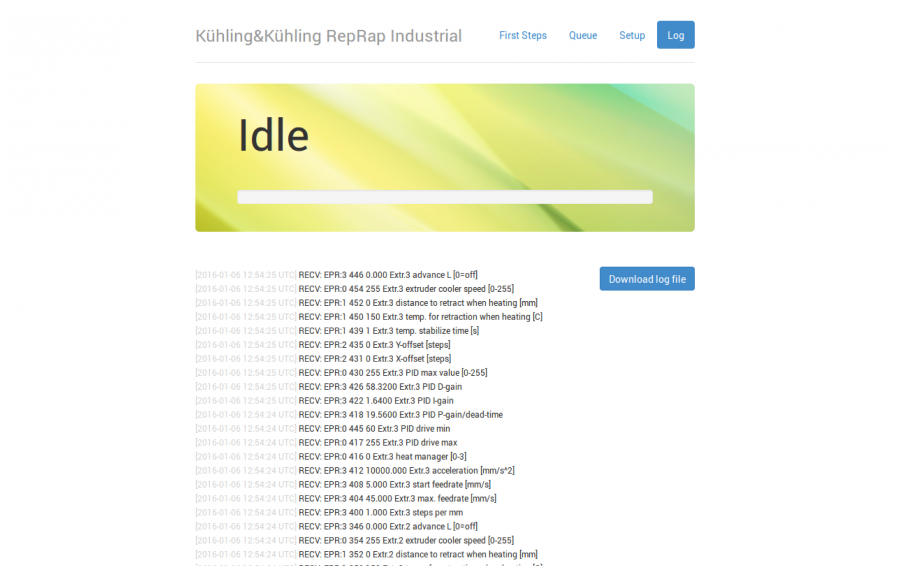
\includegraphics[width=.7\linewidth]{./img/wi_log_1.png}
  \caption{Download the log-file for support requests via the Log screen.}
\end{figure}